\section{Spezifikation der Anwendung}
In diesem Kapitel werden die Anforderungen an das System und die daraus resultierenden Anwendungsfälle beschrieben.
Anschließend wird eine System-Abgrenzung vorgenommen, sowie auf die inhaltliche Gestaltung der Anwendung eingegangen.
\subsection{Anforderungen}
Die Kernanforderung an das System ist es, dem Benutzer zu ermöglichen, sich Artikel anzuschauen und diese bestellen zu können.
Darüberhinaus soll es einem Administrator möglich sein, neue Artikel anzulegen oder bestehende zu löschen.
Dafür ist die Implementierung eines Rollensystems nötig, um die Benutzergruppen unterscheiden zu können.
Für die Bestellung von Artikeln ist es nötig, dass sich ein Benutzer in der Anwendung registrieren und seine persönlichen Daten angeben kann.
Um eine Bestellung aufzugeben muss sich der registrierte Benutzer am System anmelden können.
Die detaillierte Beschreibung der dafür benötigten Anwendungsfälle findet sich in Kapitel \ref{usecases}.
\subsection{Nichtfunktionale Anforderungen}
Die Anwendung sollte von allen gängigen Browsern in neueren Versionen sowie auf mobilen Geräten darstellbar sein.
Sensible Daten, wie die persönlichen Daten der Anwender, müssen vor unbefugtem Zugriff geschützt sein.
Im Fehlerfall soll der Benutzer über Hinweise darauf aufmerksam gemacht werden.
Dabei sollen interne Fehlermeldungen des Servers, sowie unverständliche Fehlercodes sollen vor dem Anwender verborgen werden.
Um die Benutzerfreundlichkeit der Anwendung zu sichern, sollte sich die Antwortzeit des Servers in einem vertretbaren Rahmen bewegen (Richtwert 3 Sekunden).
\subsection{Hauptanwendungsfälle}\label{usecases}
Das folgende Diagramm zeigt die Anwendungsfälle für den Benutzer und Administrator, sowie die jeweils beteiligten System-Komponenten.
Die Anwendungsfälle werden im Anschluss im Einzelnen betrachtet.
\begin{figure}[ht!]
	\centering
	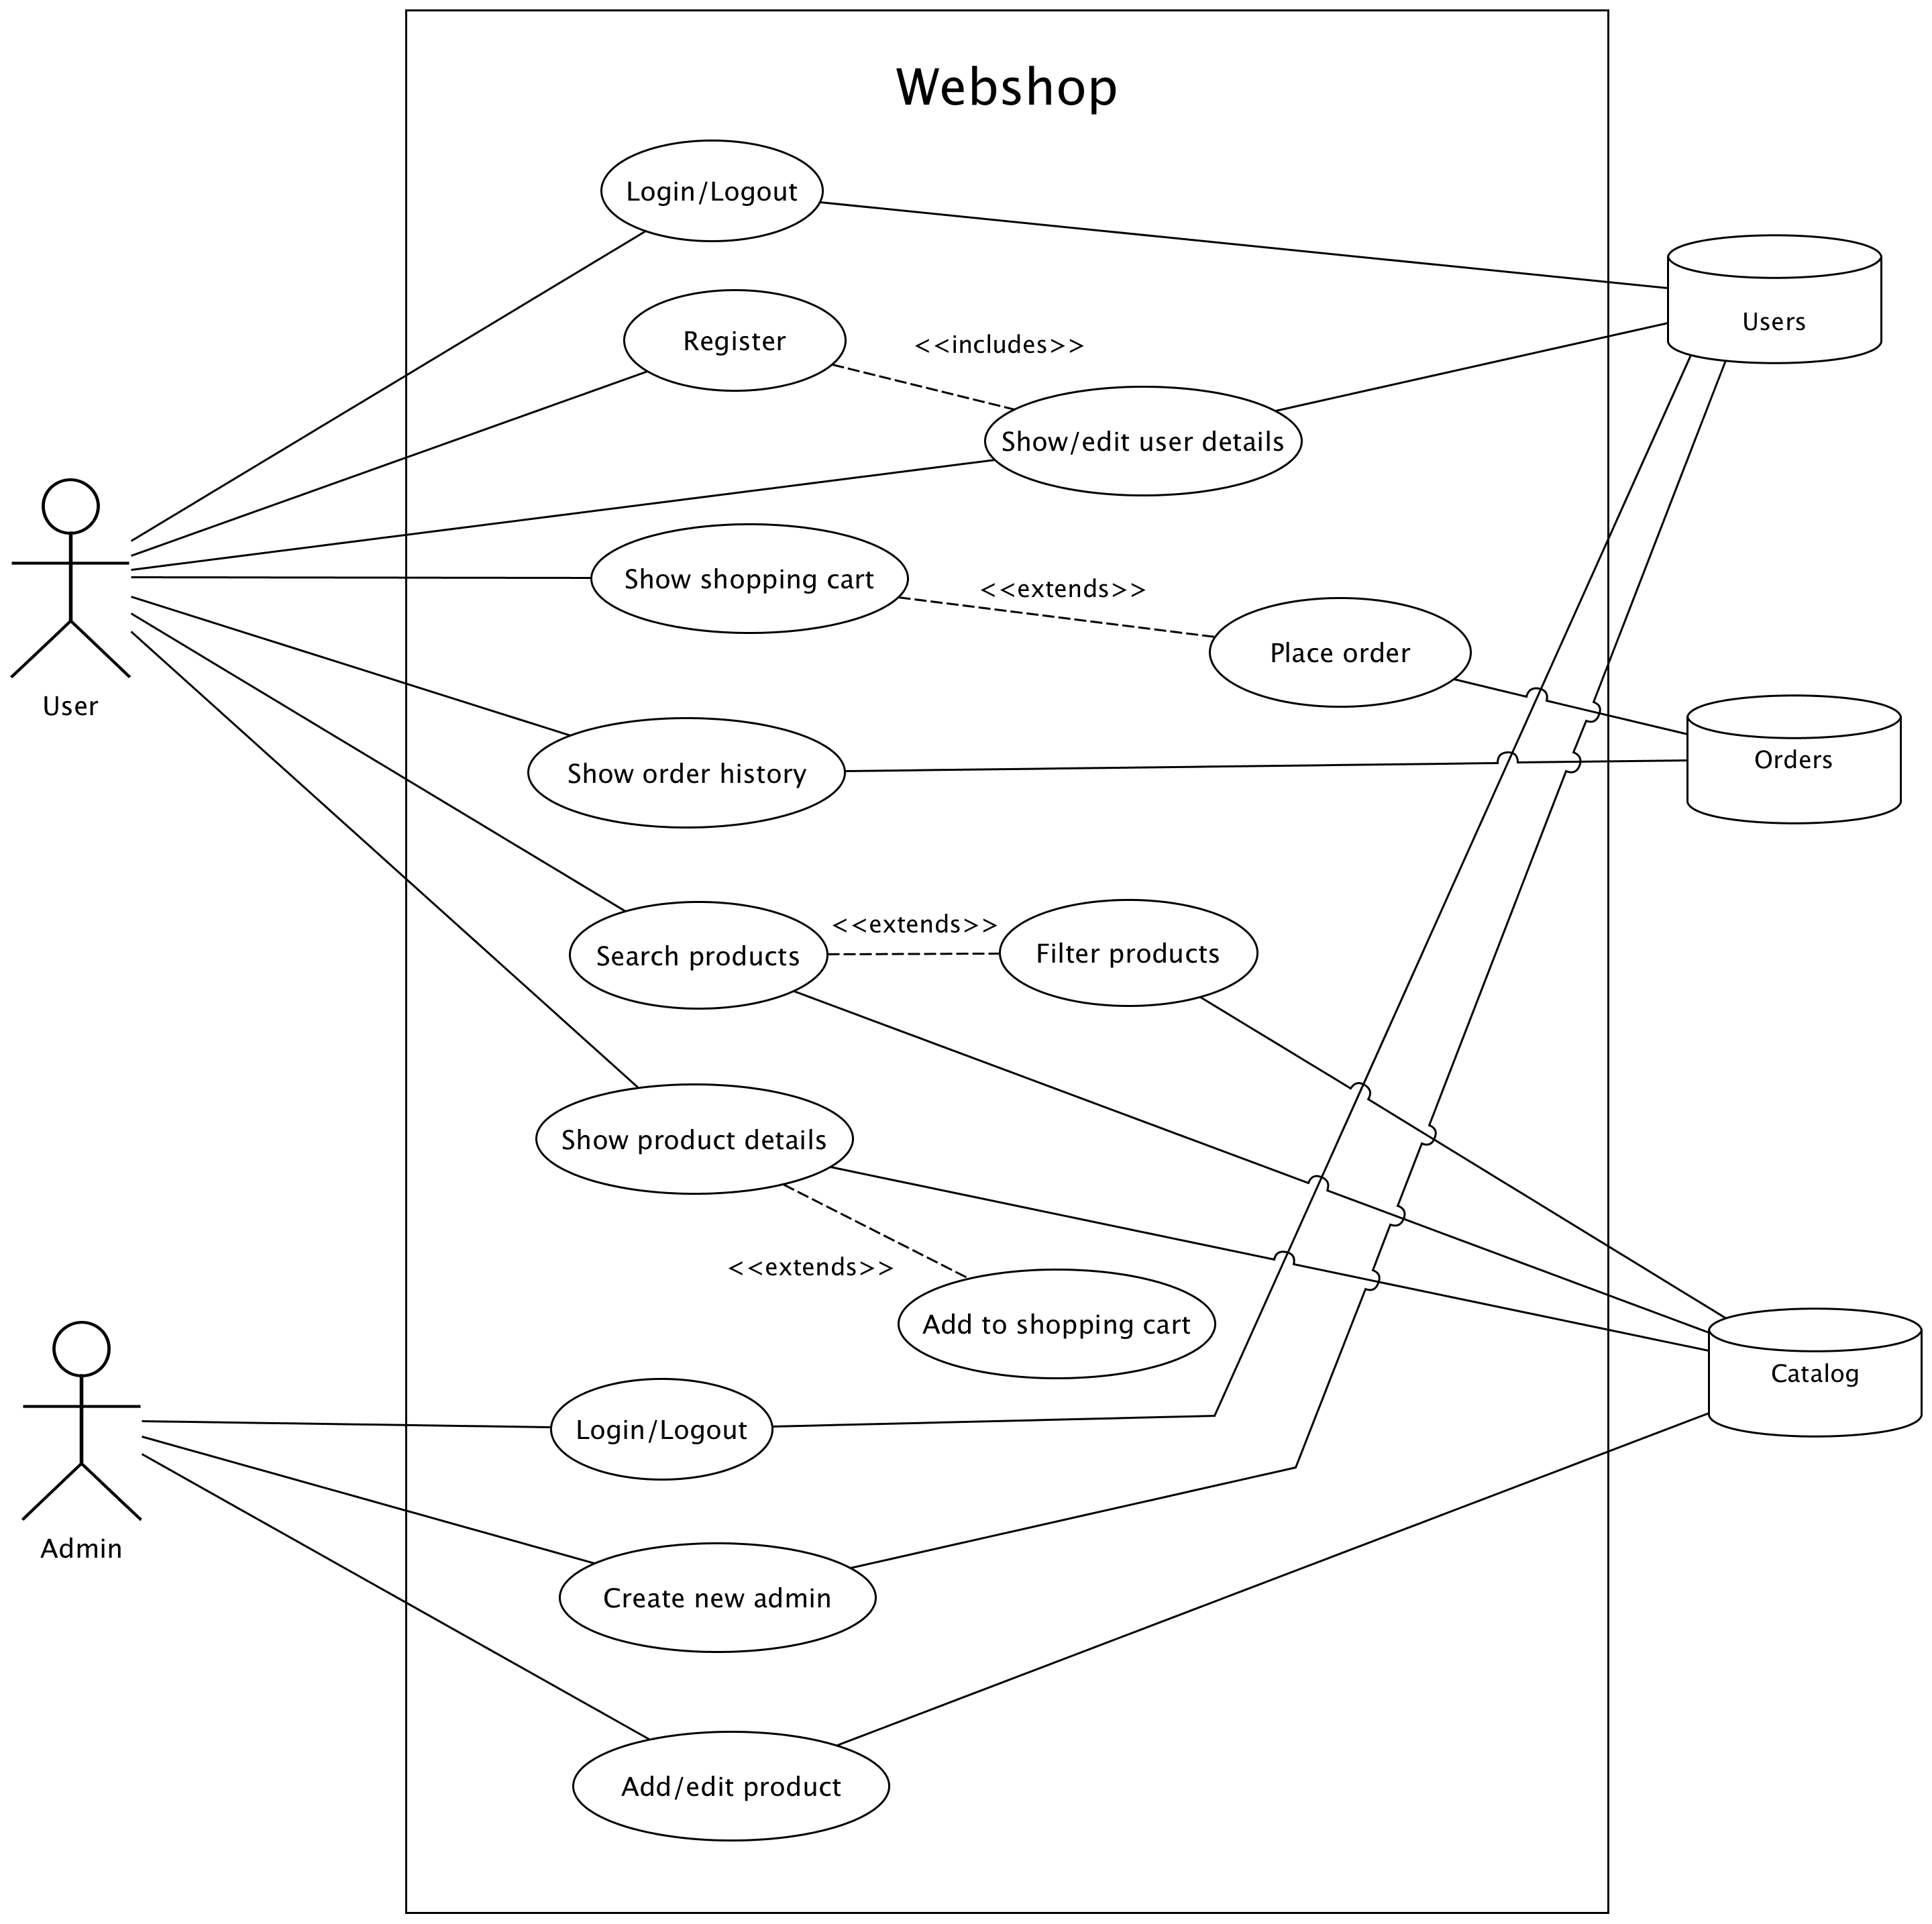
\includegraphics[width=\linewidth]{bilder/kap4/use_cases}
	\caption{}
	\label{fig:usecases}
\end{figure}

\subsubsection{Benutzer- bzw. Kunden-Anwendungsfälle}
\paragraph{Register}
Ein Benutzer soll sich durch Angabe seiner Email-Adresse, einem Passwort, sowie persönlichen Daten beim System registrieren können


\subsubsection{Administrator-Anwendungsfälle}
\subsection{System-Abgrenzung}
Diagramm, Grenzen stecken
\subsection{Inhaltliche Definition}
Wolle